\section{Analysis}
\label{sec:analysis}
\subsection{Regression analysis}
For experimentA1,
Plot a scatter chart with $\sqrt{gh}$ as the horizontal coordinate 
and x as the vertical coordinate based on the data from Table \ref{t1}.
And a regression analysis and linear fit was performed on the data, 
as shown in \autoref{ExperimentA1} and results in \autoref{table4}.

Take the average of 
the data and take it into equation \eqref{6} to get $C_v=\frac{slope}{2}$.
The final $C_v$ is 0.955.

For experiment A2, it is the same as experiment A1, with the horizontal 
coordinates replaced by $\sqrt{h}$ and the vertical coordinates replaced by Q
the data of regression analysis is in \autoref{ExperimentA2}
and results in \autoref{table5}.

Use equation \eqref{13} to caculate the $C_d=\frac{Slope}{A_0\sqrt{2g}}$
and the final $C_d$ is 0.615 (3mm)
and 0.8816 (6mm).

\begin{figure}[h]
    \centering
    \begin{minipage}[t]{0.49\textwidth}
        \centering
        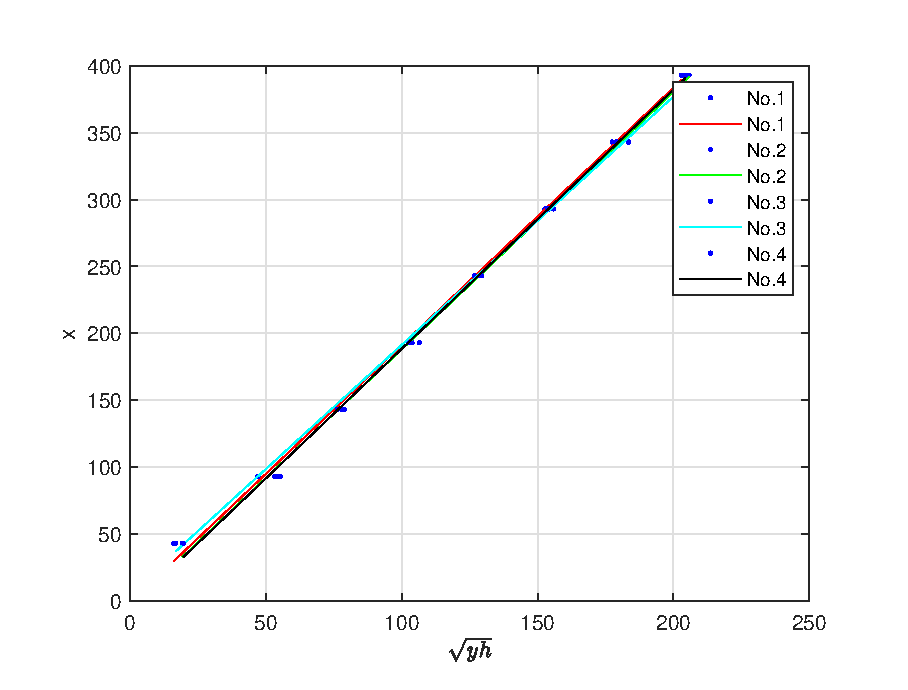
\includegraphics[width=1.12\linewidth]{Results/1.eps}
        \caption{ExperimentA1}
        \label{ExperimentA1}
        (Unit:mm)
    \end{minipage}
    \begin{minipage}[t]{0.49\textwidth}
        \centering
        \includegraphics[width=1.12\linewidth]{Results/A2.eps}
        \caption{ExperimentA2}
        \label{ExperimentA2}
       (Unit:$\sqrt{m}$ and $m^3/s$)
    \end{minipage}
\end{figure}

\begin{minipage}{\textwidth}
    \centering
\begin{minipage}[t]{0.49\textwidth}
    \makeatletter\def\@captype{table}
    \centering
    \scalebox{0.9}{
    \begin{tabular}{l|ll} 
        \hline
            & Slope    & R-square \\ \hline
        1 & 1.923 & 0.9968   \\
        2 & 1.923 & 0.9976   \\
        3 & 1.855 & 0.9985   \\
        4 & 1.936 & 0.998   \\ \hline          
    \end{tabular}} 
    \caption{result of A1 regression analysis}
    \label{table4} 
\end{minipage}
\begin{minipage}[t]{0.49\textwidth}
    \makeatletter\def\@captype{table}
    \centering
    \scalebox{0.9}{
    \begin{tabular}{l|ll}
        \hline
            & Slope    & R-square \\ \hline
        3mm & 0.00001924 & 0.9955   \\
        6mm & 0.0001103 & 0.9811   \\ \hline
        \end{tabular}}
    \caption{result of A2 regression analysis}
    \label{table5} 
\end{minipage}
\end{minipage}


%\begin{table}[h]
%    \centering
%    \begin{tabular}{l|ll}
%    \hline
%        & Slope    & R-square \\ \hline
%    3mm & 0.00001924 & 0.9955   \\
%    6mm & 0.0001103 & 0.9811   \\ \hline
%    \end{tabular}
%    \caption{result of A2 regression analysis}
%    \label{table5}
%\end{table}

\subsection{Error analysis}

$\bullet$ Inaccurate recording of water trajectory to the sheet 
due to not looking horizontally at the top point of the needle.

$\bullet$ Inaccurate calculation of the flow rate due to residual 
water in the measuring cylinder.

$\bullet$ When calculating the flow rate, errors caused by the stopwatch timing not being fully 
synchronised with the water collection time.

\FloatBarrier